\clearpage
% \begin{landscape}
\section{Comparator design}
% \begin{xltabular}{\textwidth}{YYY}
%     \hline
%     Peak power & Area efficiency & Transistor count \\
%     \hline
%     \qty{68.189}{\uW} &  \qty{103.011}{\percent} & 6 \\
%     \hline    
%     \caption{Comparator parameters}
% \end{xltabular}
\subsection{Schematic design}
Comparator design commences with reproducing the schematic design in \cref{fig:schematic} in Virtuoso's schematic editor,
and setting up a simulation to verify the schematic functions correctly. 
\begin{figure}[H]
    \centering
    \begin{subfigure}[t]{0.39\columnwidth}
        \centering
        \includegraphics[width=\textwidth]{./figures/comparator/schematic.png}
        \caption{Schematic}\label{fig:comparatorschematic}
    \end{subfigure}    
    \hfill
    \begin{subfigure}[t]{0.59\columnwidth}
        \centering
        \includegraphics[width=\textwidth]{./figures/comparator/tb.png}
        \caption{Test bench}\label{fig:comparatortb}
    \end{subfigure}    
    \vskip\baselineskip
    \begin{subfigure}[b]{\columnwidth}
        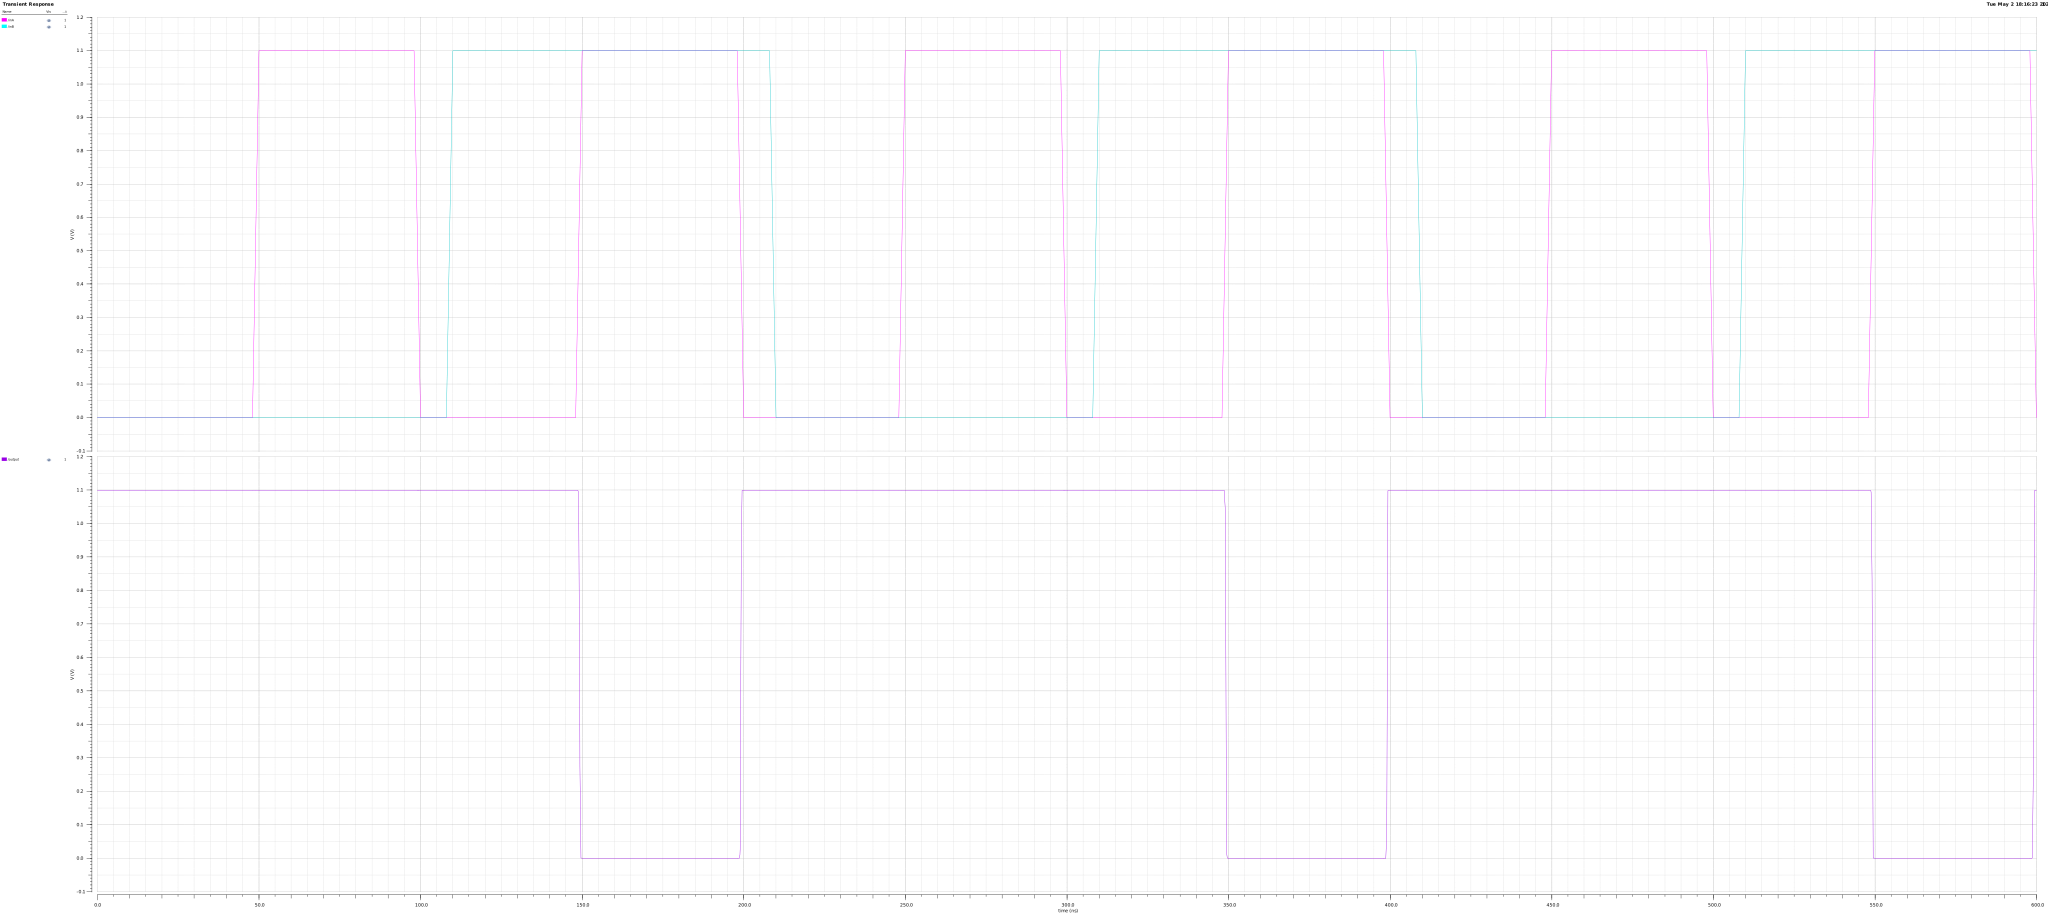
\includegraphics[width=\columnwidth]{./figures/comparator/plot-schematic.png}
        \caption{Simulation}\label{fig:comparatorplotschematic}
    \end{subfigure}
    \caption{Comparator schematic}
\end{figure}
% \end{landscape}
The simulation indicates the correct outputs for the given binary inputs. There are many instances 
in the simulation where transient undesirable outputs occur. For example, output E rises briefly, 
sometimes not even completely, when G falls and L rises at the same time. 
This is due to two reasons. In the design, a NOR gate was opted for to select the outputs rather 
than an XOR. Secondly, the rise and fall of the test bench simulation signals fall within the 
threshold voltage of the MOSFETs used. To counteract this, enough time for outputs to settle 
needs to be provided for the outputs to settle, or the comparator output can be latched 
so the output only updates on the edge of a clock. For the purposes of this design, the 
settling time will be determined after the layout is complete. 
\subsection{Layout}
The standard cell height allows for efficient routing, with vertical connections within a 
cell on the metal 3 layer, and horizontal connections between cells on metal 4 layer. 
Finally, pins and power are exposed on metal 5 layer. The pins run the height of the comparator,
so it can be connected from either end. The power rails run on metal 3, and are exposed 
at each horizontal end to metal 5. 

The cells share a well and implants, allowing them to be butted up extremely close; they can even 
be overlapped. The placement report
calculates area efficiency to be \qty{102.233}{\percent}, requiring a chip area of \qty{19.365}{\um\squared}.
\begin{landscape}
\begin{figure}[H]
    \centering
    \begin{subfigure}[t]{\columnwidth}
        \includegraphics[width=\columnwidth]{./figures/comparator/layout.png}
        \caption{Layout}\label{fig:comparatorlayout}
    \end{subfigure}    
    \vskip\baselineskip
    \begin{subfigure}[b]{\columnwidth}
        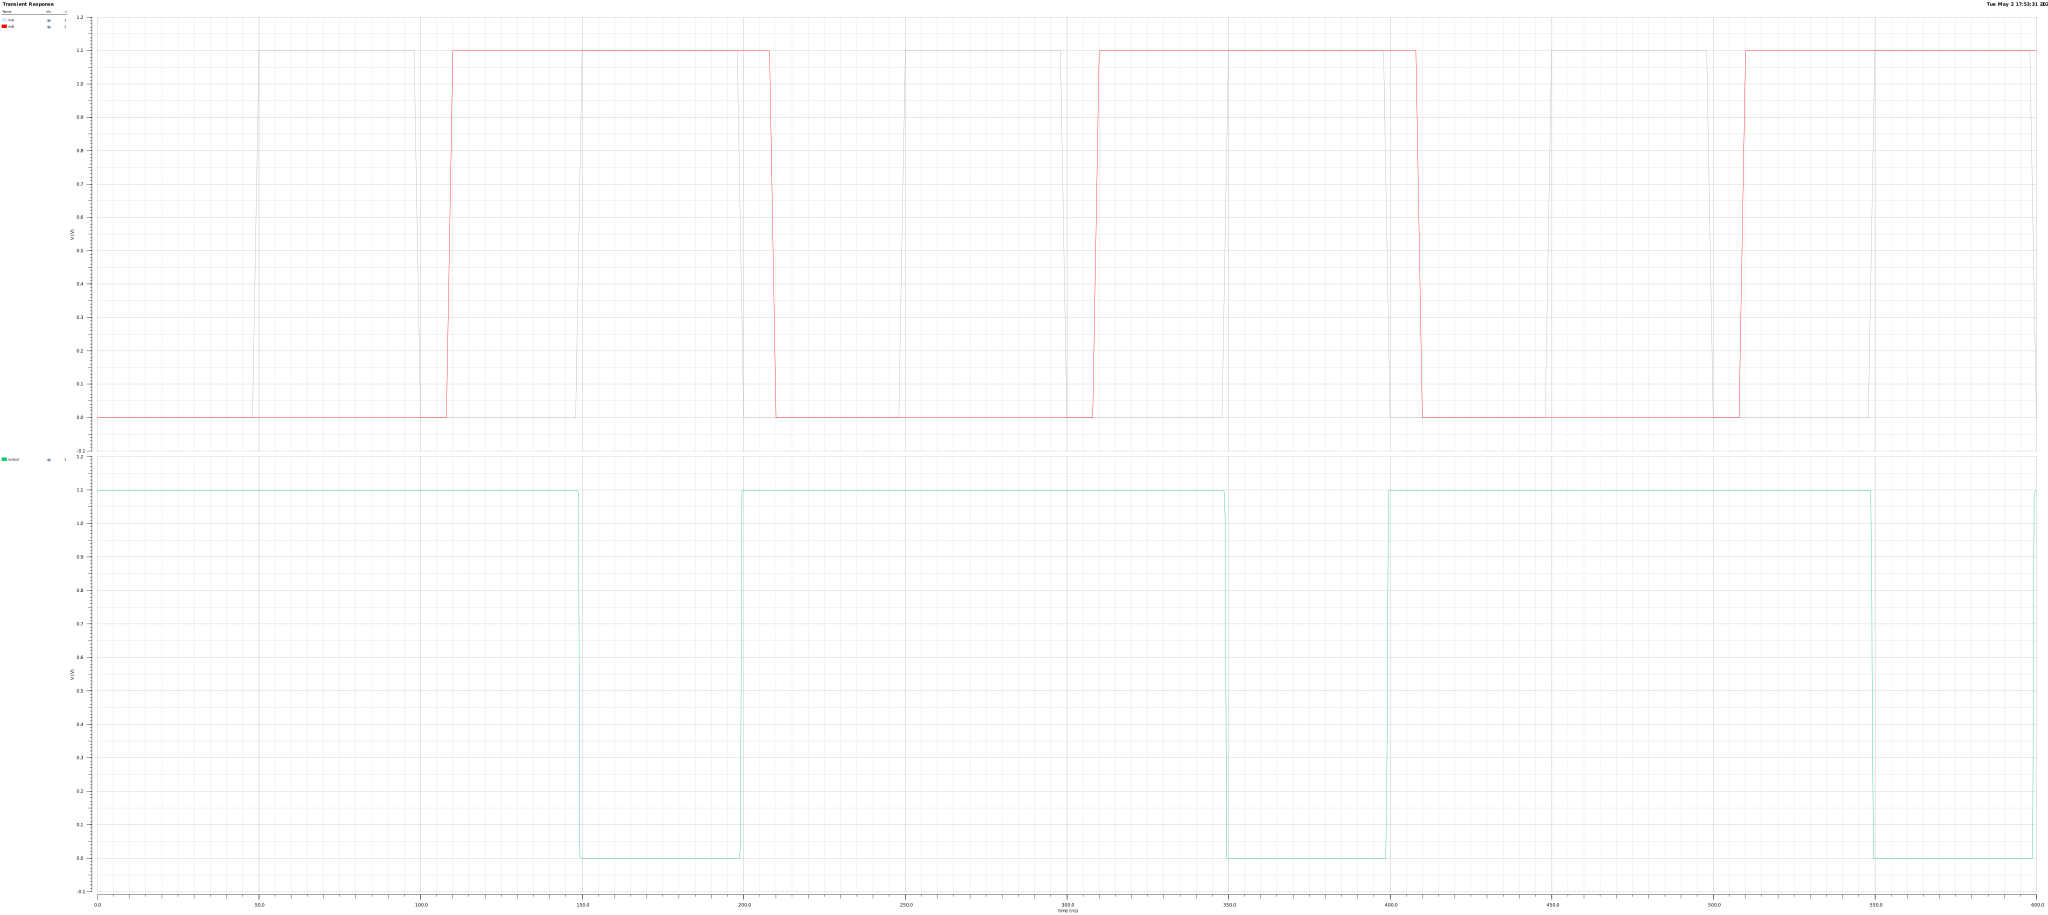
\includegraphics[width=\columnwidth]{./figures/comparator/plot-layout.png}
        \caption{Simulation}\label{fig:comparatorplotlayout}
    \end{subfigure}
    \caption{Comparator layout}
\end{figure}
\end{landscape}

\subsection{Power}
The peak dynamic power dissipation is \qty{68.189}{\uW} and occurs during switching of outputs. 
There does not appear to be a greater level of dissipation due to all outputs being high simultaneously,
suggesting that switching the NOR gate on G and E for an XNOR would have little benefit. 
\begin{figure}[H]
    \centering
    \includegraphics[width=0.95\textwidth]{./figures/comparator/pwr-outputs.png}
    \caption{Power dissipation during switching}\label{fig:comparatorpower}
\end{figure}

\subsection{Delay}
The comparator responds \qty{150}{\ps} after the input reaches \qty{50}{\percent} of vSupply (\qty{0.55}{\V}), and 
settles after an additional \qty{200}{\ps}. Considering settling time for transient outputs, readings 
are available from the comparator after, at earliest \qty{350}{\ps}, or comfortably after \qty{400}{\ps}. 
This suggests a maximum possible clock speed of \qty{2.857}{\GHz}.
\begin{figure}[H]
    \centering
    \includegraphics[width=0.95\textwidth]{./figures/comparator/sim-response-layout.png}
    \caption{Transient output}\label{fig:comparatortransient}
\end{figure}
